\section{Computational Ingredients\label{sec:PPcompset}}


\subsection{Model Space and Interaction}
The model space ($\calM$ of section~\ref{sec:splitting}), that is used
to perform the calculations presented below, consists of harmonic oscillator
states including the following shells
 $1s\frac{1}{2}$, 
 $1p\frac{3}{2}$, 
 $1p\frac{1}{2}$, 
 $1d\frac{5}{2}$, 
 $1d\frac{3}{2}$, 
 $2s\frac{1}{2}$, 
 $1f\frac{7}{2}$, 
 $1f\frac{5}{2}$, 
 $2p\frac{3}{2}$ and
 $2p\frac{1}{2}$.
The adopted size parameter was $b=1.768$~fm. The use of harmonic oscillators 
is convenient because of the Talmi-Moshinsky transformation that is used 
to transform to relative and center-of-mass coordinates 
(\cf\ chapter~\ref{chap:ppknock}). 
As such, they are
also adopted in the calculation of the G-matrix as well as the defect functions,
that have been  calculated by the procedure described by 
M\"uther and Sauer\cite{MS93a}.

Having defined the oscillator shell model space 
the G-matrix elements and defect 
wave functions are computed from the Bethe-Goldstone equation (\ref{eq:BGEP}). 
From (\ref{eq:BGEP}) it can be noted that the G-matrix elements are 
energy-dependent. This energy-dependence has been taken into account 
in chapter~\ref{chap:SPECFAC} by 
including its main effect, \viz\ the strength reduction of the main peaks of 
the single-particle propagator.

It should be expected that the G-matrix elements are only little dependent on 
the specific $NN$-interaction from which one starts\cite{MS93a}, 
since all realistic 
$NN$-interactions have been fitted to experimental scattering data and 
therefore have similar T-matrix elements. The defect wave functions on the 
other hand, may differ considerably because different short-range (repulsive) 
forces may yield similar scattering at low energies (up to a few hundred 
MeV or momenta $\onglt 1$~fm$^{-1}$).

With these arguments in mind we shall also produce some results using the 
correlation functions calculated in variational calculations by 
Clark\cite{Cl81} to describe the SRC and using the Dressed RPA (DRPA) 
amplitudes calculated with the 
G-matrix to account for long-range correlations. 
In fact, for all the calculations the DRPA amplitudes are calculated 
with a G-matrix derived from the Bonn-C potential\cite{Ma89}.

In this work calculations, which use defect functions
derived from Reid soft-core (RSC),  Bonn-A and Bonn-C meson exchange potentials
to describe the SRC, will be compared. 

\subsection{One-Body Green's Function in the Dressed RPA Calculation}
The shell model two-body removal amplitudes are obtained by solving the 
Dressed RPA equations for the two-body propagator, as discussed in 
section~\ref{sect:ppRPA}. This method is chosen because it incorporates the 
reduction of the two-body removal amplitudes by the mechanism which also 
reduces the spectroscopic factors for one-nucleon removal. The latter have 
been well investigated experimentally\cite{Leu94} and therefore it would in 
principle be possible to introduce this experimental evidence into the 
calculations. This is not done here, but instead the quite reasonable 
one-body Green's functions, calculated in chapter~\ref{chap:SPECFAC}, will be 
used. This implies that the reduction of the two-body spectral function is 
probably not strong enough. For instance, the product of the 
$1p\threehalf$ and $1p\half$ spectroscopic factors is 
$0.76*0.77$ in the calculation, while using the experimental spectroscopic 
factors (fig.~\ref{fig:Leus}) one obtains 
$(0.63\pm{0.05})*(0.65\pm{0.05})$. 
The main aim of the next sections is, however, to investigate the 
gross features of the strength as a function of the excitation energy of the 
final nucleus and to compare the 
high-momentum parts obtained with different $NN$-interactions.

\section{Defect Functions and Correlation Functions\label{sec:defect}}
Initial studies of short-range correlations were 
for practical reasons limited to central ones. Clark\cite{Cl81} 
has provided correlation functions in nuclear matter 
with analytical trial forms
for the 
Kallio-Kolltveit\cite{KK64} (KK) and the  Omhura-Morita-Yamada\cite{OMY56} 
(OMY) potentials. 
The analytical forms used are given by
%
	\begin{eqnarray}
		f_{KK}(r_{12}) 
	&=& 
		\left[
		1 - e^{ -\mu( r_{12}-c ) }
		\right]
		\left[
		1 + \gamma e^{ -\mu( r_{12}-c ) }
		\right] 
	\;\; 
	;
	\;\;
		r_{12} > c
	\label{eq:KK}
	\\
	&& \mbox{ $c=0.4$ fm, $\mu=2.20$ and $\gamma=1.572$. }
	\nonumber \\[10pt]
		f_{OMY}(r_{12}) 
	&=& 
		\left[
		1 - e^{ -\mu^2( r_{12}-c )^2 }
		\right]
		\left[
		1 + \gamma e^{ -\mu^2( r_{12}-c )^2 }
		\right] 
	\;\; 
	;
	\;\;
		 r_{12} > c
	\label{eq:OMY}
	\\
	&& \mbox{ $c=0.6$ fm, $\mu=1.118$ and $\gamma=2.078$. }
	\nonumber 
	\end{eqnarray}
%
Both correlation functions are defined to vanish for $c<r_{12}$ and are plotted
in fig.~\ref{fig:KKOMY}.
With these functions, correlated wave functions are composed,
according to (\ref{eq:corrfunc}), that can be used in the spectral function
(\ref{eq:CRSF}).
%%%%%%%%%%%%%%
\begin{figure}
\centerline{\epsfig{ file=figures/KKOMY.ps, width=8cm }
}
\vspace{0.5cm}
\caption[]{Correlation functions for the KK (\ref{eq:KK}) (solid line) and OMY 
(\ref{eq:OMY}) (dotted line) potentials. The thick dashed line is the 
correlation function calculated by Gearhart and Dickhoff\cite{GDPR95}.
\label{fig:KKOMY}
}
\end{figure}
%%%%%%%%%%%%%%

In recent years more elaborate forms for the correlation functions, 
including spin-orbit and tensor operators (\cf\ table~\ref{tab:operators}),
have been applied\cite{CFFL92,CFF94}. 
Recently, Gearhart calculated a correlation function
for relative $l=0$ states
with the self-consistent Green's functions method\cite{GDPR95}. 
This function is also displayed in fig.~\ref{fig:KKOMY}.

\subsubsection{Defect Functions}
In ref.~\cite{MS93a} defect functions have been calculated by solving the 
Bethe-Goldstone equation (\ref{eq:BGEP}) within $^{16}$O for the Reid Soft 
Core 
(RSC) potential. These functions are calculated directly in momentum space. 
Therefore, they cannot be compared immediately with the correlation functions. 
Furthermore, the Fourier transform of these defect functions should be compared
with a full correlation function (containing all the operators of 
table~\ref{tab:operators}), not only a central correlation function. Below
a comparison is made between defect 
functions calculated with different potentials and the correlation functions
that have already been calculated by Clark\cite{Cl81}.

The defect functions that will be used here are calculated
by M\"uther\cite{MuPrive95}, using the methods described in ref.~\cite{MS93a} 
for the One Boson Exchange Bonn-A
 and Bonn-C\cite{MuPrive95,Ma89} potentials. They are
plotted in fig.~\ref{fig:defectAll}.
%%%%%%%%%%%%%%
\begin{figure}
\centerline{%
\hspace{-1mm}%
\epsfig{ file=figures/deffuncs.ps, width=11.3cm }
}
\caption[]{Defect functions (\ref{eq:def}) calculated for different $(NN)$ 
potentials. The solid curves are calculated with the Bonn-A potential, the
thick dotted curves with Bonn-C and the dashed curves with the Reid Soft Core
potential. The first line contains the $^1S_0$ (left) and the $^1P_1$ (right) 
defect function. On the second line, the $^3S_1$ and $^3P_0$ defect functions
are given. On the third line the $^3P_1$ and $^3P_2$ functions are shown.
The last line contains the tensor defect functions ${^3S_1}-{^3D_1}$ (left), 
that contributes to the $^3S_1$ partial wave. On the lower
right the (${^3P_2}-{^3F_2}$) defect wave functions
are shown.
\label{fig:defectAll}
}
\end{figure}
%%%%%%%%%%%%%%

The connection with the correlation functions is made by the observation
that the correlated wave function calculated with the defect function 
(\ref{eq:def2}) equals the expression with the correlation function 
(\ref{eq:corrfunc})
%
	\begin{equation}
		\Psi(r)
	=
		\Phi(r) + \chi(r)
	=
		{\cal O}(r) \Phi(r)
	\;.
	\end{equation}
%
For $T=1$ the correlation operator is
%
	\begin{equation}
		{\cal O}(r_{12})
	=
		f_c(r_{12})
	+
		f_\sigma(r_{12})
		\gvec{\sigma}_1\cdot\gvec{\sigma}_2
	+
		f_{lS}(r_{12})
		\rvec{l}\cdot\rvec{S} 
	+
		f_t(r_{12})
		\hat{S}_{12}
	\;,
	\end{equation}
%
where the tensor operator $\hat{S}_{12}$ is given by the expression
 $3(\gvec{\sigma}_1\cdot\hat{\rvec{r}}_{12})$
\mbox{$(\gvec{\sigma}_2\cdot\hat{\rvec{r}}_{12})$} 
$-$
\mbox{$\gvec{\sigma}_1\cdot\gvec{\sigma}_2$}.
To disentangle all the different components in the correlated wave function
the following matrix elements are needed for  proton-proton (T=1) wave 
functions
%
	\begin{eqnarray}
		&\ME< \Phi_{l'}^{S' J}| {\bf 1} |\Phi_{l}^{S J}>&
	= 
		\delta_{ll'} \delta_{SS'}
	\nonumber \\ 
		&\ME< \Phi_{l'}^{S' J}|  
		\gvec{\sigma}_1\cdot\gvec{\sigma}_2
		|\Phi_{l}^{S J}>&
	= 
		\delta_{ll'} \delta_{SS'}
		(2S(S+1)-3)
	\nonumber \\ 
		&\ME< \Phi_{l'}^{S' J}|  
		\rvec{l}\cdot\rvec{S} 
		|\Phi_{l}^{S J}>&
	= 
		\delta_{ll'} \delta_{SS'}
		\half( J(J+1) - l(l+1) - S(S+1) )
	\nonumber \\ 
		&\ME< \Phi_{l'}^{S' J}|  
		\hat{S}_{12}
		|\Phi_{l}^{S J}>&
	= 
		\delta_{S1}
		\delta_{S'1}
		2\sqrt{30}
		(-)^{J+1}
		\sqrt{2l+1}
		\sqrt{2l'+1}
	\nonumber \\
	&& 
		\times
		\zesJ( J, 1, l', 2, l, 1 )
		\drieJ( l', l, 2, 0, 0, 0 )
	\nonumber 
	\;.
	\end{eqnarray}
%
These formulas can be applied to find the correlated wave function for 
different quantum numbers $l$, $S$ and $J$. Using the partial wave notation
 $^{2S+1}l_J$ for $l=S, P, D, F$, the correlated waves can be written as
%
	\begin{subeqnarray}
		\Psi(^1S_0) 
	&=&
		\left(
		f_c  -3f_\sigma 
		\right)
		\Phi(^1S_0)
	\slabel{eq:Phi1S0} \\ 
		\Psi(^3P_0) 
	&=&
		\left(
		f_c + f_\sigma  -2 f_{lS} -4 f_t  
		\right)
		\Phi(^3P_0)
	\slabel{eq:Phi3P0} \\ 
		\Psi(^3P_1) 
	&=&
		\left(
		f_c + f_\sigma  - f_{lS} +2 f_t  
		\right)
		\Phi(^3P_1)
	\slabel{eq:Phi3P1} \\ 
		\Psi(^3P_2) 
	&=&
		\left(
		f_c + f_\sigma  + f_{lS} -\sfrac{2}{5} f_t  
		\right)
		\Phi(^3P_2)
		+ 6\sqrt{6} f_t \Phi(^3F_2)
	\slabel{eq:Phi3P2} \\ 
		\Psi(^1D_2) 
	&=&
		\left(
		f_c  -3 f_\sigma 
		\right)
		\Phi(^1D_2)
	\slabel{eq:Phi1D2} \\ 
		\Psi(^3F_2) 
	&=&
		\left(
		f_c  + f_\sigma -8 f_{lS} -\sfrac{8}{5} f_t
		\right)
		\Phi(^3F_2)
		+ 6\sqrt{6} f_t \Phi(^3P_2)
	\slabel{eq:Phi3F2} 
	\end{subeqnarray}
%
The correlation functions can be extracted, if the defect functions are 
transformed to the coordinate space by means of a Fourier-Bessel transformation.
For instance, (\ref{eq:Phi1S0}) then yields
%
	\begin{equation}
		\tilde{f}_c(r) - 3f_\sigma (r)
	=
		\frac {\chi_{^1S_0}(r)}
		      {R_{00}(r)}
	\label{eq:CFextr}
	\;,
	\end{equation}
%
where $\tilde{f}_c$ is defined as $f_c -1$. 
Since the sum of (\ref{eq:Phi3P0}), three times (\ref{eq:Phi3P1}) 
and five times  (\ref{eq:Phi3P2}) 
is independent of $f_{lS}$ and $f_t$, this linear combination together with
(\ref{eq:CFextr}) is used to extract the central and spin correlation 
function $f_c$ and $f_\sigma$. 
By elimination of these from the set (\ref{eq:Phi3P0}-\ref{eq:Phi3P2}) also the 
spin-orbit and the tensor correlation functions $f_{lS}$ and $f_t$ can 
be obtained. 
These functions are plotted in fig.~\ref{fig:def2cor1}.
%%%%%%%%%%%%%%
\begin{figure}
\centerline{\epsfig{ file=figures/def2cor1.ps, width=8cm }
}
\vspace{0.5cm}
\caption[]{ The correlation function $\tilde{f}_c$($=f_c-1$) (thick solid line),
$f_\sigma$ (thin solid line), $f_{lS}$ (dotted line) and $f_t$ (dashed line) 
as obtained from the set of equations (\ref{eq:Phi3P0}-\ref{eq:Phi3P2}) 
together with (\ref{eq:CFextr}).
\label{fig:def2cor1}
}
\end{figure}
%%%%%%%%%%%%%%
%%%%%%%%%%%%%%
\begin{figure}
\centerline{\epsfig{ file=figures/cor2def/cor2def.ps, width=8cm }
}
\vspace{0.5cm}
\caption[]{Correlation functions for the Argonne $v_{14}$ potential\cite{PWP92}
\label{fig:corArg}
}
\end{figure}
%%%%%%%%%%%%%%
%%%%%%%%%%%%%%
\begin{figure}
\centerline{\epsfig{ file=figures/cor2def/defpiep.ps, width=12.5cm }
}
\vspace{0.5cm}
\caption[]{Defect functions for the correlation functions of 
fig.~\ref{fig:corArg} compared with the Reid soft-core defect functions taken 
from fig.~\ref{fig:defectAll}.
\label{fig:defectPiep}
}
\end{figure}
%%%%%%%%%%%%%%
In this figure it is shown that the old correlation functions of 
fig.~\ref{fig:KKOMY} overestimate the hole in the relative wave function 
compared
to the more realistic calculation of SRC with defect wave functions.
To test the assumption made here, that the correlation functions in the 
different partial waves 
are the same, the formulas (\ref{eq:Phi1D2}) and (\ref{eq:Phi3F2}) 
can be used to construct the ${}^1D_2$ and ${}^3F_2$ defect functions.  
The defect functions of fig.~\ref{fig:defectAll} are smaller than the 
ones constructed in this way.
The constructed ${}^1D_2$ defect function is about a 
factor two too large, while the ${}^3F_2$ differs orders of magnitude, 
but its construction with (\ref{eq:Phi3F2}) is numerically inaccurate
due to the small size of the defect function.
It seems that correlation functions, chosen to reproduce the correlations in 
the 
S-wave correctly, exaggerate correlation effects in higher $l$ components.

Recently, more elaborate calculations\cite{PWP92} have been performed to  
calculate correlation functions using a variational Monte Carlo
method\cite{PWP92}. Correlation functions for central, spin, spin-orbit and 
tensor correlations calculated with the Argonne $v_{14}$  potential are 
displayed in fig.~\ref{fig:corArg}. 
The effect of SRC in these 
functions can be investigated in the present approach if the correlation 
functions are transformed to the form of defect functions. This transformation 
that implies a Fourier-Bessel transform and algebraic manipulations described 
by (\ref{eq:Phi1S0}-\ref{eq:Phi3P2}), has been performed and the results are 
shown in fig.~\ref{fig:defectPiep}.
There is a reasonable agreement between the Reid and 
Argonne potential for high relative momenta. One should keep in mind, however,
that the calculation of the defect functions at low momenta lead to numerical 
difficulties associated with the treatment of the Pauli operator in the 
Bethe-Goldstone equation\cite{MS93a}. This could explain the discrepancy at 
low momenta.
